\part{Memory}
\frame{\partpage}

\begin{frame}{Memory Hierarchy}
\begin{figure}
	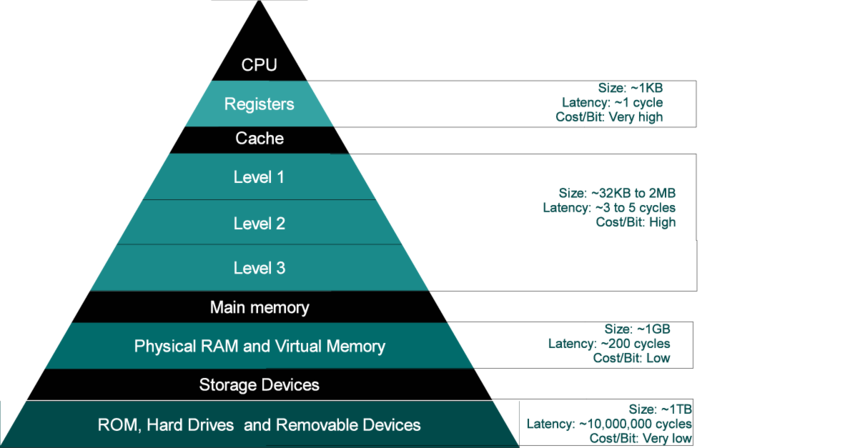
\includegraphics[width=1.0\textwidth,height=0.8\textheight]{Memory-hierarchy}  
\end{figure}
\end{frame}

\begin{frame}{Registers \& Caches}
\end{frame}

\begin{frame}{Main Memory}
\end{frame}

\begin{frame}{Storage}
\end{frame}

\begin{frame}{Memory Optimisation}
	\begin{itemize}
		\pause \item Reduce Memory footprint
		\pause \item Write algorithms which reduce memory traversal
		\pause \item Increase cache hits
		\pause \item Increase temporal coherence
		\pause \item Utilise Pre-fetching
		\pause \item Avoid patterns which break caching 
	\end{itemize}
\end{frame}

\begin{frame}{Reduce Memory Footprint}
\end{frame}

\